% C.29 AB 直径，C 圆上，∠BAC=35°
\documentclass[tikz,border=4pt]{standalone}
\usepackage{ctex}
\usepackage{amsmath}
\usetikzlibrary{calc, arrows.meta}
\begin{document}
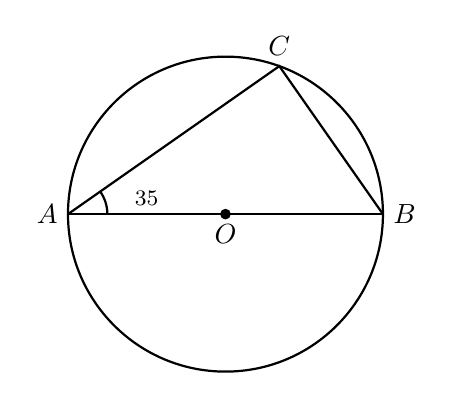
\begin{tikzpicture}[scale=1.0, thick]
  \coordinate (O) at (0,0);
  \draw (O) circle (2);
  \coordinate (A) at (-2,0);
  \coordinate (B) at (2,0);
  \coordinate (C) at ({2*cos(180-2*35)}, {2*sin(180-2*35)});
  % ∠BAC=35 inscribed in semicircle → C such that arc... place C with central angle ∠BOC=2*35=70 from B
  % Just put C at angle 70: C=(2cos70, 2sin70)
  \coordinate (C) at ({2*cos(70)}, {2*sin(70)});
  \draw (A) -- (B);
  \draw (A) -- (C) -- (B);
  % 直角 at C
  % perpendicular: draw small square at C between CA and CB
  \filldraw (O) circle (1.5pt) node[below] {$O$};
  \node[left] at (A) {$A$};
  \node[right] at (B) {$B$};
  \node[above] at (C) {$C$};
  \draw (-1.5,0) arc (0:atan2({2*sin(70)},{2*cos(70)+2}):0.5);
  \node[font=\footnotesize] at (-1.0,0.2) {$35°$};
\end{tikzpicture}
\end{document}
